% !TEX program = xelatex

\documentclass[12pt,a4paper]{article}
\usepackage[margin=2.2cm]{geometry}
\usepackage{graphicx}
\usepackage{booktabs}
\usepackage{amsmath}
\usepackage{float}
\usepackage{hyperref}
\usepackage{xcolor}
\usepackage{listings}

\lstset{
  language=Python,
  basicstyle=\ttfamily\small,
  keywordstyle=\color{blue!70!black},
  commentstyle=\color{green!40!black},
  stringstyle=\color{orange!60!black},
  showstringspaces=false,
  breaklines=true,
  frame=single,
  tabsize=4
}

% XeLaTeX 中文支持，使用 TeX Live 内置的 Fandol 字体集
\usepackage[fontset=fandol]{ctex}

\title{计算机网络专题实验七个人补充\\\large 停车场出入场系统的功能完善与问题修复说明}
\author{姓名：李祥熙\quad 班级：计算机2301 \quad 学号：2234412799}
\date{\today}

\begin{document}
\maketitle

\section*{引言：原实现存在的问题与不足}
在第一次提交验收后，我们对照指导书逐条复查了原有实现，发现系统虽然完成了“上传图片—OCR识别—入出场判定—计费—前端反馈”的核心闭环，但与指导书的必做要求仍存在以下差距：

\begin{enumerate}
  \item \textbf{取图方式不完整。}指导书要求手机客户端分别提供“拍摄车牌”（调用摄像头，模拟扫描动作）与“从相册选择车牌图片”两项独立功能。原页面只有一个通用的文件选择框，未设置\texttt{capture}属性，无法明确调起手机摄像头，也没有区分两种取图入口。
  \item \textbf{缺少图片预览。}指导书实验步骤明确要求客户端在上传前预览所选图片，原页面选择文件后仅显示文件名，用户无法确认拍摄内容是否清晰、正向。
  \item \textbf{入场/出场按钮缺失。}指导书要求客户端界面包含入场/出场按钮。服务端虽然实现了\texttt{channel}通道参数（\texttt{entry}/\texttt{exit}/\texttt{auto}），但原前端从未发送该参数，所有请求都走\texttt{auto}自动模式，“重复入场”“未入场先出场”两类异常在正常操作路径下实际无法触发，业务语义不完整。
  \item \textbf{持久化字段不全。}指导书要求出入场记录持久化“车牌号、入场时间、出场时间、停车时长、费用、状态”等字段，原数据库表缺少\textbf{停车时长}字段，出场响应中也未返回时长信息。
  \item \textbf{存在若干代码缺陷。}入场时间以\texttt{str(datetime.now())}格式存储、出场时按固定含微秒格式\texttt{\%Y-\%m-\%d \%H:\%M:\%S.\%f}解析——当时间戳恰好微秒为零时格式不含小数部分，解析会抛出异常导致出场失败；上传文件按原始文件名保存，同名文件会互相覆盖；\texttt{pick\_city\_char()}函数末尾存在不可达的死代码；错误提示中列出的支持格式与实际允许的扩展名不一致。
  \item \textbf{可选优化项（加分项）基本未实现。}车位管理、管理员后台、识别缓存、上传图片定期清理、文件日志模块、多线程并发等指导书列出的加分方向均为空白。
\end{enumerate}

针对以上问题，我们对系统进行了一轮系统性的完善与修复。本补充报告按“功能修改—功能新增—缺陷修复—测试验证”的顺序说明全部改动。

\section*{一、对必做功能的修改与完善}

\subsection*{1. 拍摄车牌与相册选择分离，并增加图片预览}
前端取图区重构为两个独立按钮，分别绑定两个隐藏的\texttt{input}控件：“拍摄车牌”使用\texttt{accept="image/*" capture="environment"}直接调起手机后置摄像头，“从相册选择”不带\texttt{capture}属性以打开系统相册。任一方式选定图片后，立即通过\texttt{URL.createObjectURL()}在预览区显示缩略图，并提示文件名与大小，用户确认清晰后再上传。

\begin{lstlisting}[language=HTML]
<!-- capture=environment 调用手机后置摄像头；无 capture 则打开相册 -->
<input type="file" id="camera-input" accept="image/*"
       capture="environment" hidden>
<input type="file" id="album-input" accept="image/*" hidden>
\end{lstlisting}

\begin{lstlisting}
function onFilePicked(input, sourceName){
    const file = input.files[0];
    if (!file) return;
    selectedFile = file;
    // 图片预览
    if (previewUrl) URL.revokeObjectURL(previewUrl);
    previewUrl = URL.createObjectURL(file);
    previewImg.src = previewUrl;
    ...
}
\end{lstlisting}

\subsection*{2. 入场/出场按钮与通道参数打通}
页面第二步操作区提供“入场识别”“出场识别”“智能判断”三个按钮，点击时把对应的\texttt{channel}值（\texttt{entry}/\texttt{exit}/\texttt{auto}）随\texttt{multipart/form-data}一并提交。由此，服务端已有的通道校验逻辑真正生效：入场通道遇到在场记录返回\texttt{409 duplicate\_entry}（重复入场），出场通道找不到在场记录返回\texttt{409 exit\_before\_entry}（未入场先出场），\texttt{auto}通道保持“在场则出场、否则入场”的自动语义。上传期间三个按钮统一禁用并显示旋转进度提示，避免重复提交。

图\ref{fig:comp-ui}为完善后的移动端首页实拍截图：顶部实时显示剩余车位与当前费率；第一步为“拍摄车牌/从相册选择”双入口与预览区；第二步为入场/出场/智能判断三个通道按钮；底部为最近一次响应展示区与管理员后台入口。

\begin{figure}[H]
  \centering
  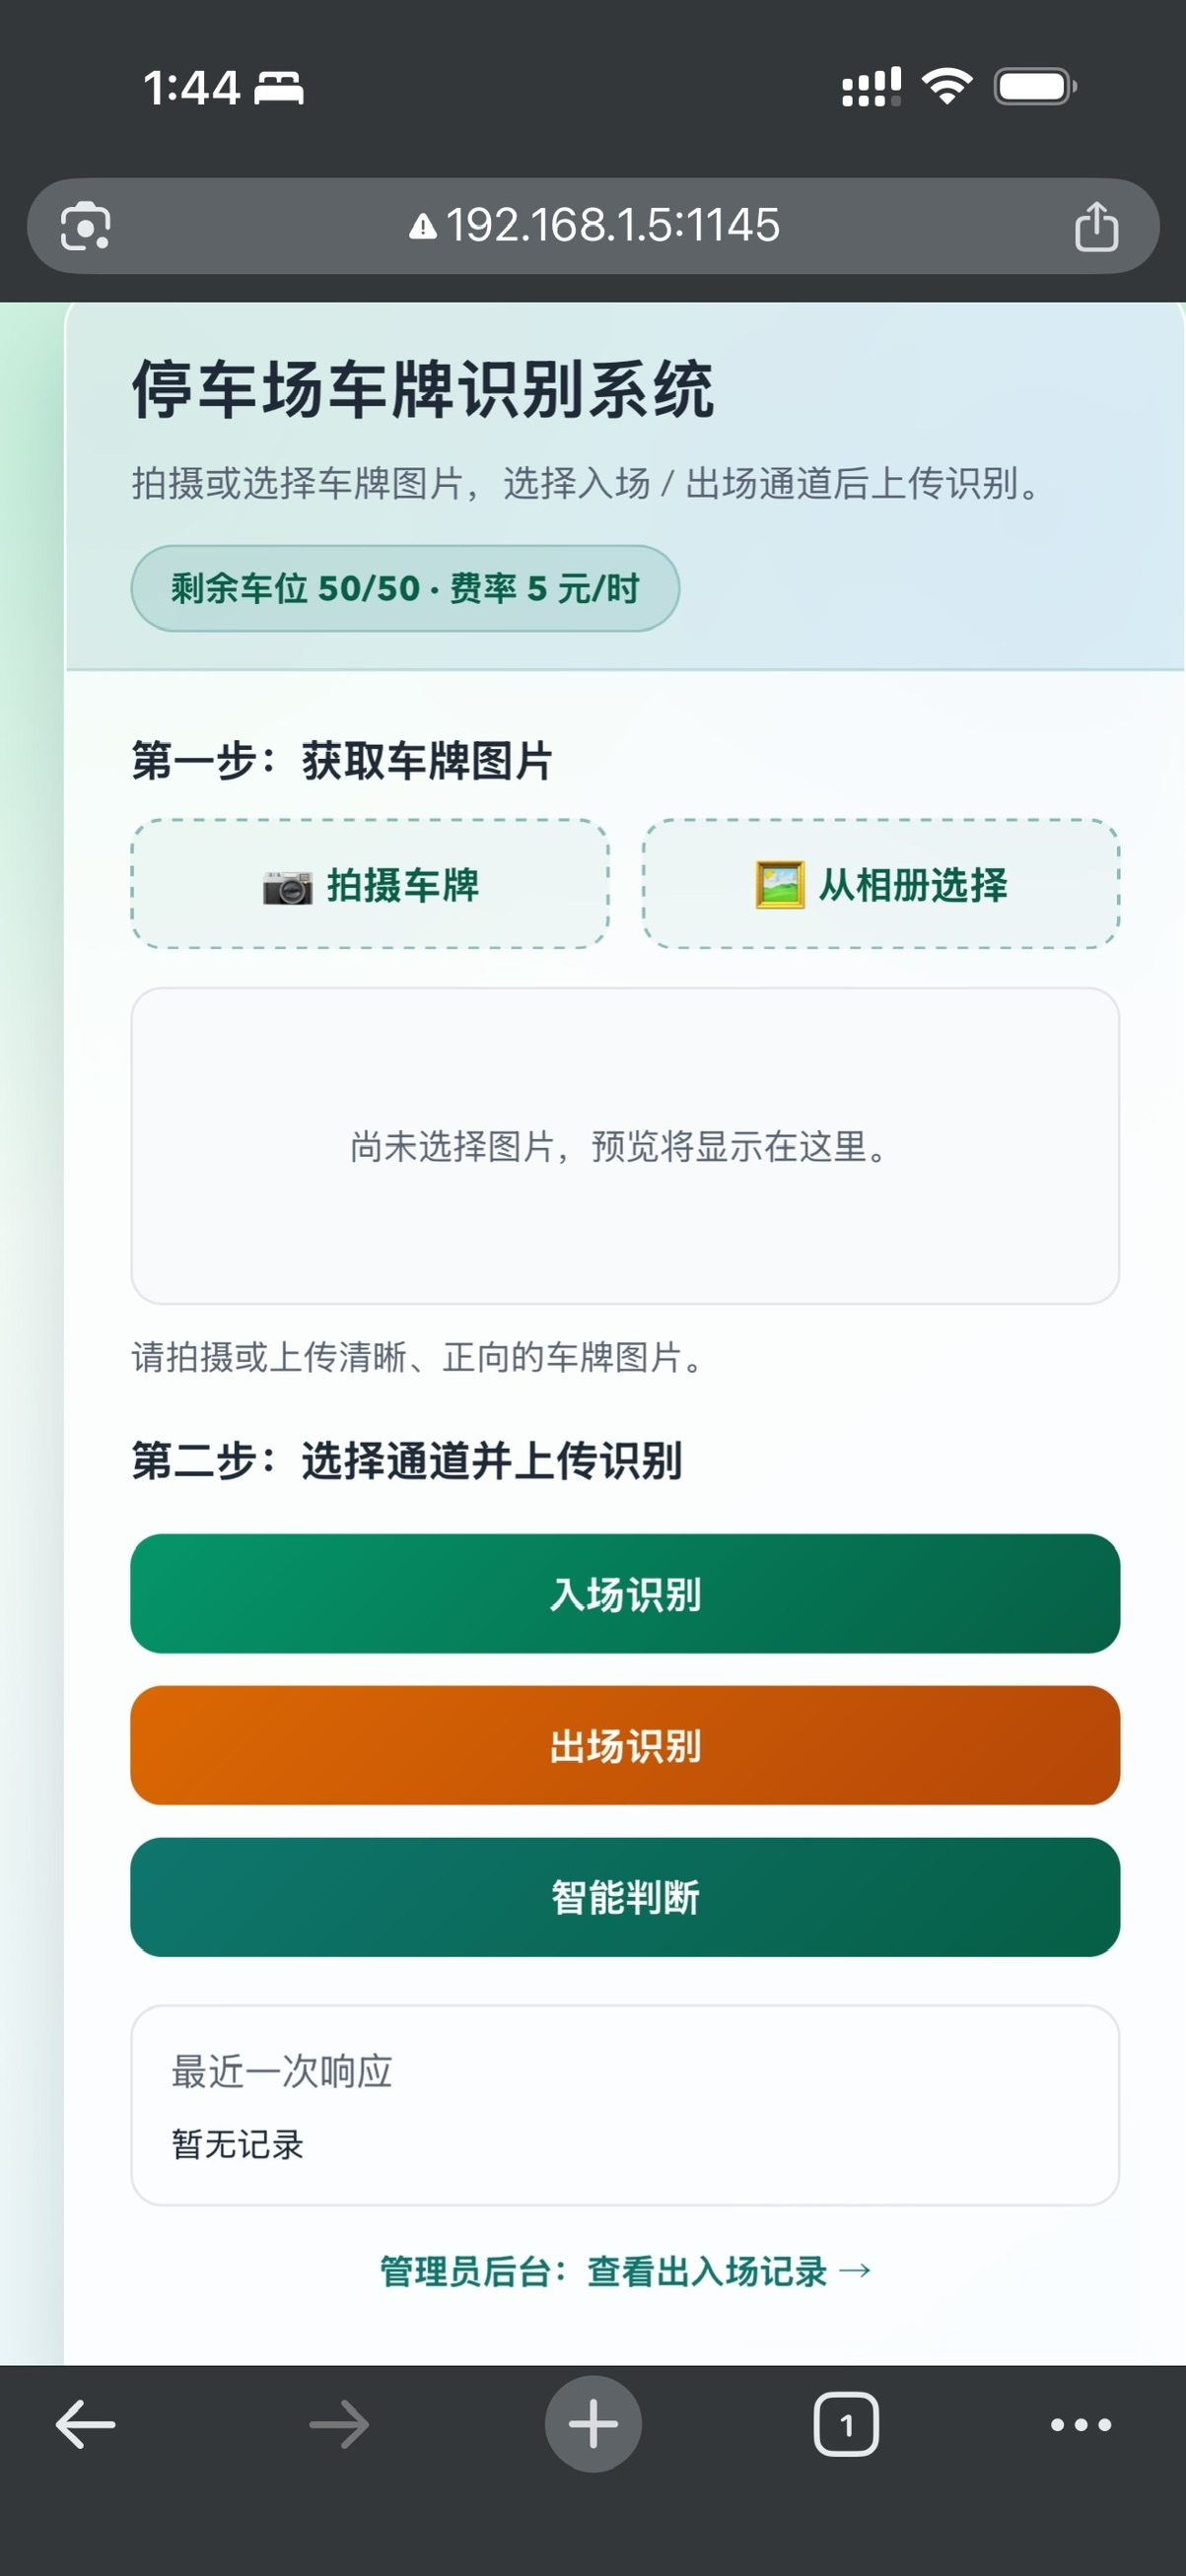
\includegraphics[width=0.5\textwidth]{image-complementary.jpeg}
  \caption{完善后的移动端首页：取图双入口、图片预览、入出场通道按钮与剩余车位展示}
  \label{fig:comp-ui}
\end{figure}

\subsection*{3. 补全停车时长持久化}
数据库表\texttt{cars}重新设计为：自增主键\texttt{id}、车牌号\texttt{plate}、入场时间\texttt{enter\_time}、出场时间\texttt{exit\_time}、\textbf{停车时长\texttt{duration\_minutes}（分钟）}、费用\texttt{fee}、状态\texttt{status}，完整覆盖指导书要求的持久化字段。为兼容已有数据，\texttt{init\_db()}会检查旧表结构并通过\texttt{ALTER TABLE}自动补列迁移。出场结算时由统一的\texttt{calc\_fee()}同时计算费用与时长并落库，出场响应也新增\texttt{duration\_minutes}与\texttt{enter\_time}字段供前端展示。

\begin{lstlisting}
def calc_fee(enter_time, exit_time, fee_per_hour):
    # 按小时线性计费，不足一小时按比例
    seconds = max((exit_time - enter_time).total_seconds(), 0)
    hours = seconds / 3600
    fee = round(hours * fee_per_hour, 2)
    duration_minutes = round(seconds / 60, 2)
    return fee, duration_minutes
\end{lstlisting}

\section*{二、新增功能（对应指导书加分项）}

\subsection*{1. 停车场车位管理}
费率与总车位数持久化在新增的\texttt{config}配置表中（默认50个车位、5元/小时）。入场前先统计在场车辆数，车位已满时拒绝入场并返回\texttt{403 lot\_full}与可读提示；入场成功的响应携带\texttt{remaining\_spots}剩余车位数。同时新增\texttt{GET /spaces}接口返回总车位、在场数、剩余车位与当前费率，前端首页顶部以徽标形式实时展示，每次上传后自动刷新。

\subsection*{2. 管理员后台}
新增网页版管理员后台，由三个接口组成：
\begin{itemize}
  \item \texttt{GET /admin}：后台主页（\texttt{templates/admin.html}），以卡片展示总车位、在场车辆、剩余车位与累计收费统计，并列出最近200条出入场记录（含停车时长），在场/离场状态以不同颜色区分。
  \item \texttt{POST /admin/config}：在线修改停车费率与总车位数，服务端校验“费率非负、车位数为正整数”，保存后即时生效。
  \item \texttt{GET /admin/export}：一键导出全部记录为收费报表CSV，表头包含车牌号、入出场时间、停车时长、费用与状态；文件带UTF-8 BOM，Excel可直接打开且中文不乱码。
\end{itemize}
另新增\texttt{GET /records}接口以JSON返回出入场记录，支持\texttt{plate}参数按车牌模糊过滤，便于程序化查询与自动化测试。

\subsection*{3. 车牌识别缓存}
对上传图片的原始字节计算MD5哈希作为缓存键，识别成功后写入内存缓存；同一图片再次上传时直接复用识别结果，跳过车牌定位与OCR全过程，显著降低重复识别的响应时间。缓存设置容量上限并加互斥锁保护，保证多线程下的一致性。

\begin{lstlisting}
image_hash = hashlib.md5(image_bytes).hexdigest()
plate = cache_get_plate(image_hash)
if plate:
    log_info(f"Plate cache hit: hash={image_hash[:12]}, plate={plate}")
else:
    ...  # 车牌定位 + 分阶段OCR
    if plate:
        cache_put_plate(image_hash, plate)
\end{lstlisting}

\subsection*{4. 上传图片定期清理}
服务启动时立即执行一次清理，并启动守护线程每30分钟扫描一次\texttt{uploads/}目录，删除修改时间超过24小时的历史图片，避免长期运行导致磁盘占用过大；清理动作与结果均写入日志。

\subsection*{5. 日志模块}
将原先基于\texttt{print}的日志替换为标准\texttt{logging}模块：同一条日志同时输出到控制台与滚动日志文件\texttt{server.log}（单文件上限2MB、保留3个备份），格式统一为“级别—时间—内容”，覆盖每次请求的候选区域、OCR中间结果、业务判定、异常与清理动作，便于事后排查与复现。

\subsection*{6. 多线程并发支持}
Flask以\texttt{threaded=True}多线程模式启动，支持多台手机同时上传；EasyOCR的懒加载初始化与识别缓存的读写均通过互斥锁保护；每个请求独立创建SQLite连接并设置超时，避免并发写库冲突。

\section*{三、缺陷修复}

\begin{enumerate}
  \item \textbf{出场时间解析崩溃。}原实现按固定格式 \%Y-\%m-\%d \%H:\%M:\%S.\% f解析入场时间，而 str(datetime.now()) 在微秒恰好为零时不含小数部分，会触发\texttt{ValueError}导致出场请求直接失败。修复：入库时间统一格式化为\texttt{\%Y-\%m-\%d \%H:\%M:\%S}，解析时由 parse\_stored\_time() 依次尝试新旧两种格式，兼容历史数据。

\begin{lstlisting}
def parse_stored_time(value):
    # 兼容两种历史格式: 带/不带微秒
    for fmt in (TIME_FORMAT, "%Y-%m-%d %H:%M:%S.%f"):
        try:
            return datetime.strptime(value, fmt)
        except ValueError:
            continue
    raise ValueError(f"无法解析时间: {value}")
\end{lstlisting}

  \item \textbf{上传文件同名覆盖。}原实现直接以\texttt{secure\_filename}后的原始文件名保存，两次上传同名图片会互相覆盖，且并发上传存在竞争。修复：保存时统一加“年月日\_时分秒\_微秒”时间戳前缀，保证文件名唯一。
  \item \textbf{死代码清理。}删除\texttt{pick\_city\_char()}函数中位于\texttt{return}语句之后、永远不可达的多余\texttt{return None}。
  \item \textbf{错误提示与实际行为不一致。}允许的扩展名集合包含\texttt{webp}，但错误提示只列到\texttt{gif}；同时“空文件名”分支的响应缺少统一的\texttt{error}错误码字段。两处均已修正，所有错误响应统一为“\texttt{error}错误码 + \texttt{msg}中文提示 + 语义化HTTP状态码”的结构。
  \item \textbf{文件保存与内容校验解耦。}原实现先\texttt{file.read()}读取字节做解码校验，再\texttt{seek(0)}后调用\texttt{file.save()}二次落盘；现改为校验通过后直接把已读入内存的字节写盘，避免流状态相关的隐患。
\end{enumerate}

\section*{四、接口变更汇总}

\begin{table}[H]
  \centering
  \begin{tabular}{lll}
    \toprule
    接口 & 方法 & 说明 \\
    \midrule
    \texttt{/} & GET & 移动端首页（重构：取图双入口、预览、通道按钮） \\
    \texttt{/upload} & POST & 识别接口（前端现已实际传递\texttt{channel}参数） \\
    \texttt{/spaces} & GET & \textbf{新增}：车位与费率信息 \\
    \texttt{/records} & GET & \textbf{新增}：出入场记录查询（支持车牌过滤） \\
    \texttt{/admin} & GET & \textbf{新增}：管理员后台页面 \\
    \texttt{/admin/config} & POST & \textbf{新增}：修改费率与总车位数 \\
    \texttt{/admin/export} & GET & \textbf{新增}：导出收费报表CSV \\
    \bottomrule
  \end{tabular}
  \caption{本次完善后的完整接口列表}
\end{table}

出场成功的响应在原有\texttt{plate}、\texttt{type}、\texttt{fee}、\texttt{time}基础上新增\texttt{duration\_minutes}（停车时长）与\texttt{enter\_time}（入场时间）；入场成功的响应新增\texttt{remaining\_spots}（剩余车位）。新增错误码包括\texttt{lot\_full}（403，车位已满）与\texttt{invalid\_config}（400，后台配置非法）。

\section*{五、测试验证}
为确认改动的正确性，我们在OCR环节使用固定返回结果的桩模块替代EasyOCR（识别管线本身未改动，其正确性已由第一次实验的真实样本测试验证），对服务端进行了端到端自动化冒烟测试，共39项断言全部通过，覆盖：

\begin{enumerate}
  \item \textbf{页面要素}：首页包含摄像头取图控件（\texttt{capture="environment"}）、相册控件、预览元素与入场/出场按钮；
  \item \textbf{上传校验}：缺文件、空文件、非法扩展名、损坏图片、非法通道参数分别返回400/415等对应状态码；
  \item \textbf{业务流程}：入场成功（含剩余车位）、重复入场409、出场成功（含费用、时长、入场时间）、未入场先出场409、\texttt{auto}通道自动判定；
  \item \textbf{新增功能}：识别缓存命中、\texttt{/spaces}与\texttt{/records}（含车牌过滤）、车位满员403、出场释放车位、管理后台页面渲染、费率配置修改与非法配置拒绝、CSV导出；
  \item \textbf{缺陷回归}：带微秒的历史时间格式可正常出场结算、上传文件名唯一不覆盖、超期图片被清理线程删除、\texttt{server.log}日志文件正常写入。
\end{enumerate}

测试结果为\textbf{39 passed, 0 failed}，且真机（手机浏览器经局域网访问，见图\ref{fig:comp-ui}）验证了页面加载、车位信息拉取与整体交互均正常。

\section*{六、小结}
本次补充工作在保持“真实OCR识别 + 规则增强”识别管线不变的前提下，补齐了指导书的全部必做要求（拍摄/相册双取图、图片预览、入出场通道按钮、停车时长持久化），实现了六项加分方向（车位管理、管理员后台、识别缓存、定期清理、日志模块、多线程并发），并修复了时间解析崩溃、文件覆盖等五处缺陷。经过39项自动化断言与真机联调验证，系统功能完整、异常路径清晰，达到了指导书对功能完整性与代码健壮性的要求。

\end{document}
